\iffalse
TODO: aggiungere bibliografia
TODO: revisione generale
\fi

\chapter{Large Language Model - Cosa sono e come funzionano}

\begin{figure}[htbp]
    \centering
    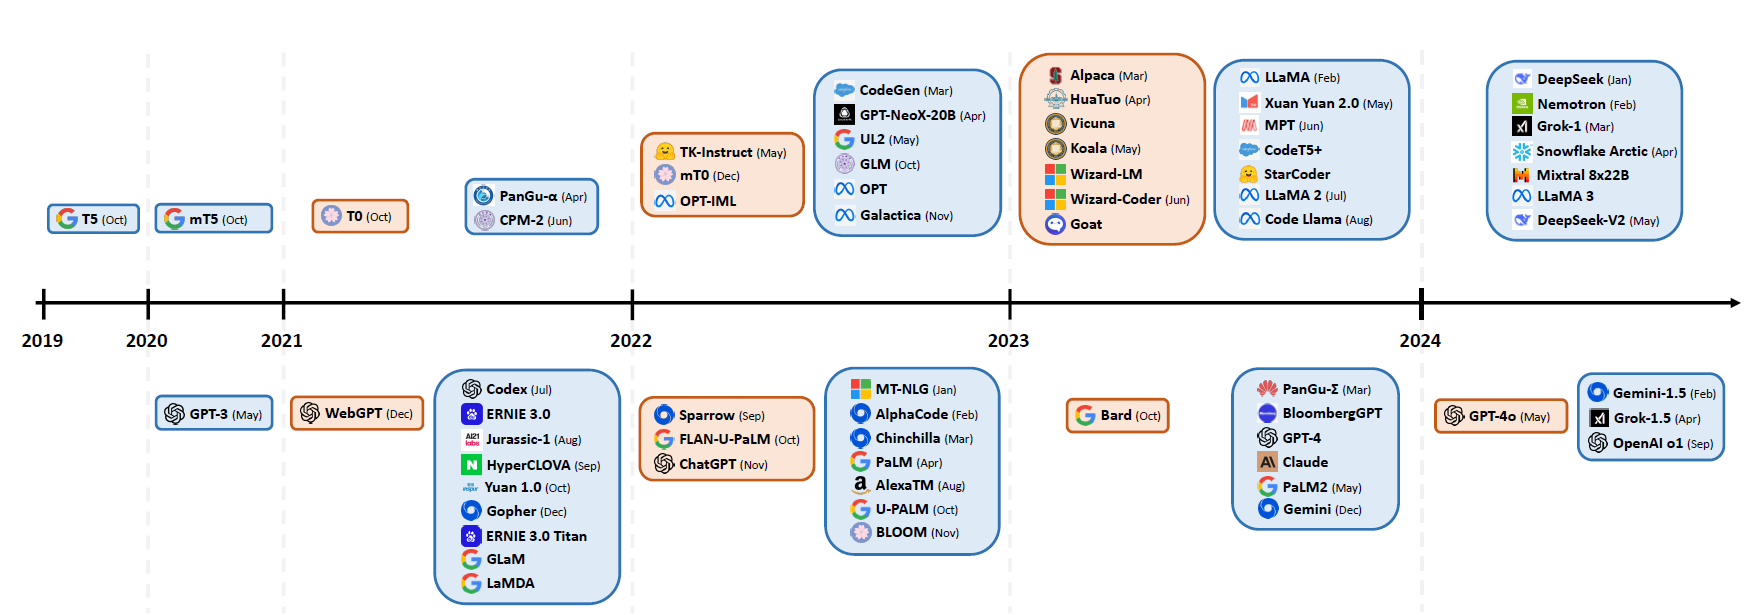
\includegraphics[width=0.9\textwidth]{../figure/llms-timeline.png}
    \caption{Cronologia dei principali \textit{Large Language Models} (LLM) sviluppati fino al 2024. 
        Sopra la linea ci sono i modelli open-source, mentre sotto ci sono quelli closed-source.
        \cite{arxiv230706435}
    }
    \label{fig:llms-timeline}
\end{figure}

\section{Introduzione}

Il linguaggio rappresenta uno strumento fondamentale per gli esseri umani, 
sia come mezzo di comunicazione e trasmissione di conoscenza, 
sia come interfaccia privilegiata per l'interazione con le macchine. 
Lo sviluppo di modelli linguistici sempre più potenti è stato quindi al centro 
della ricerca in \textit{Natural Language Processing} (NLP). 

Storicamente, si è passati da approcci \textbf{statistici} (basati su n-grammi e modelli probabilistici),
a \textbf{modelli neurali}, fino ai \textbf{modelli pre-addestrati} (\textit{Pre-trained Language Models}, PLM).
Questi ultimi, addestrati in maniera auto-supervisionata su grandi corpus testuali,
hanno introdotto il concetto di rappresentazioni generali del linguaggio, 
successivamente adattabili tramite \textit{fine-tuning} a specifici compiti \cite{devlin2019bert}\cite{peters2018elmo}\cite{lewis2019bart}.

Un punto di svolta è stato l'introduzione dei \textbf{\textit{Transformer}} \cite{chernyavskiy2021transformers}, 
che hanno reso possibile scalare i modelli a miliardi di parametri grazie al meccanismo di attenzione,
alla parallelizzazione ed alla disponibilità di hardware e dataset sempre più estesi.
Questo ha portato alla nascita dei \textbf{Large Language Models} (LLM).

\subsection{Capacità degli LLM}
Con la crescita di scala, gli LLM hanno mostrato proprietà nuove:
\begin{itemize}
    \item \textbf{Generalizzazione senza fine-tuning}: capacità di risolvere compiti mai visti 
    semplicemente a partire da una descrizione testuale (\textit{prompting}).
    \item \textbf{\textit{Zero-shot}} e \textbf{\textit{few-shot learning}}: risoluzione di compiti senza esempi (\textit{zero-shot}) 
    o con pochissimi esempi forniti nel prompt (\textit{few-shot}).
    \cite{chung2022scaling}\cite{sanh2021multitask}\cite{wang2022supernaturalinstructions}\cite{wang2022selfinstruct}\cite{ouyang2022rlhf}\cite{touvron2023llama2}
    \item \textbf{\textit{In-context learning}}: adattamento “al volo” alle istruzioni fornite nell'input.
    \item \textbf{Abilità emergenti}: ragionamento, pianificazione, decision-making, risoluzione di problemi logici,
    che non erano stati esplicitamente programmati durante l'addestramento.
    \cite{wei2022emergent}\cite{webb2023emergent}\cite{boiko2023emergent}
\end{itemize}

\subsection{Sfide e limitazioni}
Nonostante queste capacità impressionanti, gli LLM presentano limiti significativi:
\begin{itemize}
    \item \textbf{Costi computazionali ed energetici elevatissimi}, sia in fase di addestramento che di inferenza 
    (i.e.: durante l'uso effettivo del modello).
    \item \textbf{Allucinazioni}: generazione di contenuti plausibili ma in realtà falsi.
    \item \textbf{Bias e tossicità}: riflessione di stereotipi e pregiudizi presenti nei dati di addestramento.
    \item \textbf{Problemi di allineamento}: difficoltà nel seguire fedelmente l'intento umano; 
    si ricorre quindi a tecniche come \textit{instruction tuning} e \textit{reinforcement learning from human feedback} (RLHF).
    \item \textbf{Accessibilità limitata}: solo pochi attori industriali dispongono delle risorse necessarie 
    per addestrare modelli di queste dimensioni.
\end{itemize}

\newpage
\section{Funzionamento}

Illustriamo ora i concetti fondamentali per comprendere
la struttura e il funzionamento dei \textit{Large Language Models} (LLM).

\subsection{Panoramica}
Per capire come funzionano gli LLM è utile seguire il flusso informativo: il testo grezzo viene prima pre-processato e tokenizzato, i token vengono poi trasformati in rappresentazioni numeriche che attraversano una architettura di Transformer basata su meccanismi di attenzione e infine il modello viene addestrato (spesso in modo distribuito). Le diverse scelte in ciascuna di queste fasi (tokenizzazione, qualità dei dati, obiettivo di training, architettura) determinano in gran parte le capacità e i limiti del modello.

\subsection{Tokenizzazione e pre-processing dei dati}
La tokenizzazione spezza il testo in unità elementari chiamate token: possono essere singoli caratteri, sottoparole (subword) o parole complete. Le tecniche comuni (es. \textit{Byte-Pair Encoding}, \textit{SentencePiece}) cercano un compromesso tra un vocabolario piccolo e la capacità di rappresentare parole rare o morfologie complesse. Prima della tokenizzazione si eseguono operazioni di pre-processing: filtraggio della qualità, deduplicazione e rimozione di informazioni sensibili. Un buon pre-processing dei dati riduce inoltre rumore, bias e contenuti non desiderati, migliorando la generalizzazione del modello.

\subsection{Il Transformer: principio e componenti fondamentali}
Il Transformer è l'architettura alla base degli LLM moderni. Si basa su un principio chiamato \textit{self-attention}: 
nel rappresentare matematicamente i token del prompt, trasformandoli in oggetti chiamati \textit{embeddings}, si tiene conto non solo della parola isolata ma anche dell'intera frase 
nella quale si trova, aggiungendo così il contesto.

\begin{itemize}
    \item \textbf{\textit{Multi-head attention}}: il modello osserva la frase da più punti di vista contemporaneamente (più "teste") per catturare relazioni diverse, come quelle grammaticali o semantiche.
    \item \textbf{\textit{Positional encoding}}: poiché l'attenzione è insensibile alla posizione, si aggiunge un segnale posizionale per preservare l'ordine delle parole.
    \item \textbf{\textit{Feed-forward locale}}: dopo l'attenzione, ogni token viene elaborato da una piccola rete indipendente che raffina la sua rappresentazione.
\end{itemize}

Ci sono diverse tipologie di Transformer:
\begin{itemize}
    \item \textbf{\textit{Encoder-decoder}}: due parti separate, una legge l'input (\textit{encoder}) e l'altra genera l'output (\textit{decoder}). Utile per traduzione o riassunti.
    \item \textbf{\textit{Decoder autoregressivo}}: genera una parola alla volta guardando solo le parole già prodotte (utilizzato nei modelli GPT).
    \item \textbf{Architetture ibride}: combinano attenzione bidirezionale e causale per casi specifici.
    \item \textbf{\textit{Mixture-of-Experts (MoE)}}: il modello ha molti "esperti" specializzati e per ogni input ne attiva solo alcuni, migliorando l'efficienza su larga scala.
\end{itemize}

\subsection{Obiettivi di pre-training}
Gli obiettivi di addestramento definiscono cosa il modello apprende:
\begin{itemize}
    \item \textbf{\textit{Causal Language Modeling} (CLM)}: prevedere il token successivo (approccio autoregressivo).
    \item \textbf{\textit{Masked Language Modeling} (MLM)}: ricostruire token volontariamente mascherati (approccio bidirezionale).
    \item \textbf{Permutation Language Modeling}: il modello predice token in ordine permutato.
    \item \textbf{\textit{Prefix / Unified objectives}}: combinano modalità diverse per aumentare la flessibilità. La scelta dell'obiettivo influenza l'uso finale: 
    i modelli autoregressivi sono particolarmente adatti alla generazione libera, mentre i modelli basati su masking risultano efficaci 
    per rappresentazioni contestuali e compiti di classificazione.
\end{itemize}

\subsection{Leggi di scalabilità e considerazioni pratiche}
Studi empirici sulle cosiddette \emph{scaling laws} mostrano che le prestazioni migliorano in modo prevedibile all'aumentare del numero dei parametri, 
quantità di dati e risorse computazionali, spesso seguendo relazioni di tipo esponenziali. Tuttavia, aumentare solamente la quantità di dati 
senza adeguare la capacità del modello o le risorse computazionali non garantisce miglioramenti proporzionali. È quindi fondamentale bilanciare dimensione del modello, 
qualità e quantità dei dati e budget computazionale per ottenere guadagni effettivi.

\subsection{Stadi di adattamento: dal pre-training all'uso}
Il ciclo di vita di un LLM si articola tipicamente in tre fasi principali:
\begin{enumerate}
    \item \textbf{Pre-training}: apprendimento auto-supervisionato su grandi corpus testuali per acquisire conoscenze linguistiche generali.
    \item \textbf{Fine-tuning / Alignment}: adattamento a compiti specifici o preferenze umane.
    \item \textbf{Prompting / Utilizzo}: impiego diretto tramite prompt.
\end{enumerate}

In sintesi, un LLM è il risultato di una catena integrata: dati curati e tokenizzazione efficiente alimentano un'architettura Transformer che, 
tramite meccanismi di self-attention, costruisce rappresentazioni robuste. L'addestramento distribuito su larga scala con obiettivi appropriati 
modella il comportamento finale, mentre tecniche di adattamento e prompting permettono l'impiego del modello in applicazioni concrete.

\newpage
\section{\textit{Pre-training} degli LLM}

Il \textbf{\textit{pre-training}} è la fase cruciale che consente ai Large Language Models (LLM) di acquisire conoscenza linguistica generale e capacità di 
rappresentazione del testo prima di qualsiasi adattamento specifico.

\subsection{Obiettivi del Pre-training}
Gli LLM vengono addestrati in modo auto-supervisionato su grandi corpus testuali con diversi obiettivi di ottimizzazione:
\begin{itemize}
    \item \textbf{Causal Language Modeling (CLM)}: il modello predice il prossimo token dato il contesto precedente. 
    \item \textbf{Masked Language Modeling (MLM)}: alcuni token vengono mascherati e il modello deve ricostruirli.
    \item \textbf{Permutation Language Modeling}: il modello predice token in ordine permutato.
    \item \textbf{Prefix Language Modeling}: viene scelto un prefisso casuale e il modello deve predire i token successivi.
    \item \textbf{Unified Language Modeling}: combina strategie diverse per aumentare la flessibilità.
\end{itemize}

\subsection{Dataset di Addestramento}
La qualità e la varietà dei dati di pre-training sono fondamentali. Le principali categorie di dataset includono:
\begin{itemize}
    \item \textbf{Corpus web}: testi raccolti da siti web, ad esempio \textit{Common Crawl}.
    \item \textbf{Enciclopedie e risorse strutturate}, come Wikipedia.
    \item \textbf{Libri e testi lunghi}, ad esempio \textit{BooksCorpus}.
    \item \textbf{Forum e codice}, inclusi dataset come \textit{The Pile}, \textit{Github}, \textit{StackExchange}.
\end{itemize}
Prima dell'addestramento, i dataset subiscono processi di filtraggio e deduplicazione.

\subsection{Sfide del Pre-training}
L'addestramento degli LLM pone sfide di tipo computazionale e metodologico:
\begin{itemize}
    \item \textbf{Costo computazionale}: i modelli con centinaia di miliardi di parametri richiedono settimane di addestramento su supercomputer 
    con migliaia di GPU.
    \item \textbf{Efficienza dei dati}: la disponibilità di dati di alta qualità è limitata.
    \item \textbf{Rumore e bias}: i dati web contengono rumore, contenuti tossici e bias culturali che vengono appresi dal modello.
    \item \textbf{Controllo della qualità}: è necessario implementare filtri e curare la selezione delle fonti.
\end{itemize}

\subsection{Tendenze Recenti}
Le ricerche recenti nel pre-training hanno introdotto innovazioni quali:
\begin{itemize}
    \item \textbf{Adattamento multilingue}: uso di corpus in centinaia di lingue.
    \item \textbf{Addestramento multimodale}: integrazione di testo con immagini, audio o codice.
    \item \textbf{Data Mixture Optimization}: selezione ponderata delle fonti testuali per massimizzare la qualità dell'apprendimento.
    \item \textbf{Continual Pre-training}: estendere progressivamente le conoscenze aggiornando i modelli con nuovi dati.
\end{itemize}

\newpage
\section{Fine-tuning e Adattamento degli LLM}

Dopo il pre-training, gli LLM vengono tipicamente sottoposti a una fase di \textbf{adattamento}, che ne affina le capacità su compiti specifici o 
ne migliora l'allineamento con le intenzioni umane. Questo capitolo descrive i metodi principali di fine-tuning, le strategie di efficientamento 
dei parametri e le tecniche di allineamento.

\subsection{\textit{Supervised Fine-tuning} (SFT)}
Consiste nell'addestrare ulteriormente l'LLM su un dataset etichettato per compiti specifici (es. traduzione, classificazione, QA).
\begin{itemize}
    \item Viene usato per adattare un modello generalista a un dominio ristretto (es. medicina, diritto).
    \item Può essere effettuato con dataset relativamente piccoli rispetto al pre-training.
    \item Rischia di causare \textit{catastrophic forgetting}, ossia perdita delle conoscenze generali.
\end{itemize}

\subsection{Instruction Tuning}
Gli LLM vengono ottimizzati per comprendere e seguire istruzioni in linguaggio naturale.
\begin{itemize}
    \item Basato su dataset di tipo \textit{prompt-response}, costruiti manualmente o tramite crowdsourcing.
    \item Introduce la capacità di rispondere in modo coerente a comandi generali senza ulteriori adattamenti.
\end{itemize}

\subsection{Reinforcement Learning from Human Feedback (RLHF)}
Il \textbf{RLHF} rappresenta una tecnica fondamentale per allineare i modelli alle preferenze umane.
\begin{enumerate}
    \item Si raccoglie un dataset di risposte generate dal modello valutate da esseri umani.
    \item Si addestra un \textbf{modello di reward} che impara a prevedere la valutazione di cui prima.
    \item L'LLM viene ulteriormente ottimizzato con tecniche di reinforcement learning.
\end{enumerate}
Questo approccio è stato utilizzato da, ad esempio, ChatGPT.

\subsection{Domain Adaptation}
Gli LLM possono essere specializzati in domini specifici:
\begin{itemize}
    \item \textbf{Continued Pre-training}: ulteriore addestramento su corpus specializzati.
    \item \textbf{Fine-tuning supervisionato su task di dominio}.
    \item \textbf{Approcci ibridi}: combinazioni di pre-training e PEFT ( \textit{Parameter-Efficient Fine-Tuning} ).
\end{itemize}

\subsection{Multitask e Meta-apprendimento}
Oltre al fine-tuning per singoli compiti, sono stati esplorati approcci che 
mirano a una maggiore generalizzazione:
\begin{itemize}
    \item \textbf{\textit{Multi-task Fine-tuning}}: addestramento simultaneo su più compiti.
    \item \textbf{Meta-apprendimento}: insegnare al modello ad adattarsi rapidamente a nuovi compiti con pochi esempi.
\end{itemize}

\subsection{Alignment Tuning}
Per garantire sicurezza, utilità e rispetto delle preferenze etiche, 
si introducono strategie di \textbf{alignment}:
\begin{itemize}
    \item \textbf{\textit{Constitutional AI}}: uso di principi predefiniti come linee guida per il comportamento del modello.
    \item \textbf{\textit{Self-critique e revisione}}: i modelli generano e valutano autonomamente le proprie risposte.
    \item \textbf{Feedback multimodale}: estensione del RLHF con segnali da immagini, audio o interazioni più complesse.
\end{itemize}

\newpage
\section{Tecniche di Prompting e In-Context Learning}

Dopo il pre-training e l'eventuale fine-tuning, i Large Language Models (LLM) 
vengono tipicamente utilizzati tramite la formulazione di \textbf{prompt}, cioè sequenze di input testuali che guidano la generazione.

\subsection{Zero-shot Prompting}
Nel \textbf{\textit{zero-shot prompting}} il modello riceve soltanto una descrizione del compito 
in linguaggio naturale, senza esempi.
\begin{itemize}
    \item Dimostra la capacità di generalizzazione appresa durante il pre-training.
    \item Funziona bene per compiti semplici e largamente rappresentati nei dati di training.
    \item È la modalità più naturale di interazione con un LLM.
\end{itemize}

\subsection{Few-shot Prompting e In-Context Learning (ICL)}
Nel \textbf{few-shot prompting}, al modello vengono forniti alcuni esempi 
di input-output all'interno del prompt. Consente al modello di inferire lo schema del compito e adattarsi in tempo reale.
Questo comportamento è noto come \textbf{\textit{in-context learning}} (ICL).

\subsection{Prompt Engineering}
La formulazione del prompt influenza drasticamente la qualità delle risposte.
Sono dunque emerse tecniche sistematiche di \textbf{prompt engineering}:
\begin{itemize}
    \item \textbf{Instruction-style prompts}: forniscono istruzioni chiare e contestualizzate.
    \item \textbf{Template-based prompting}: utilizzo di schemi predefiniti per generare input coerenti.
    \item \textbf{Role prompting}: assegnazione di un “ruolo” al modello (es. “Sei un medico con decenni di esperienza…”).
\end{itemize}

\subsection{Prompting per il Ragionamento}
Gli LLM possono essere spinti a mostrare capacità di ragionamento tramite prompt opportuni.
Le tecniche principali sono:
\begin{itemize}
    \item \textbf{\textit{Chain-of-Thought} (CoT)}: incoraggia il modello a produrre spiegazioni passo-passo.
    \item \textbf{\textit{Self-Consistency}}: genera più catene di ragionamento e seleziona la risposta più frequente.
    \item \textbf{\textit{Tree-of-Thought} (ToT)}: esplora diversi percorsi di ragionamento, con possibilità di backtracking.
    \item \textbf{\textit{Generated Knowledge Prompting}}: il modello produce prima conoscenza di supporto, poi la usa per rispondere.
\end{itemize}

\subsection{Multi-turn Prompting}
Alcuni compiti complessi richiedono interazioni iterative con il modello.
\begin{itemize}
    \item \textbf{Single-turn prompting}: il modello riceve tutte le informazioni in un unico prompt.
    \item \textbf{Multi-turn prompting}: l'interazione è suddivisa in più turni, 
    con feedback e aggiustamenti progressivi. Questo approccio è alla base degli \textbf{agenti autonomi} basati su LLM.
\end{itemize}

\subsection{Tecniche Avanzate di Prompting}
Sono state sviluppate ulteriori strategie per aumentare l'affidabilità:
\begin{itemize}
    \item \textbf{Prompt Chaining}: suddividere un compito complesso in più sotto-compiti concatenati.
    \item \textbf{Automatic Prompt Generation}: generazione automatica di prompt efficaci 
    tramite ottimizzazione o meta-modelli.
    \item \textbf{\textit{Retrieval-Augmented Prompting}}: combinazione con sistemi di recupero documentale 
    per fornire contesto aggiornato e ridurre le allucinazioni.
\end{itemize}

\newpage
\section{Benchmarking e Valutazione degli LLM}

La valutazione degli LLM è una componente cruciale per misurarne le capacità, 
confrontare modelli diversi e guidare lo sviluppo futuro. 
Questo capitolo analizza le principali metriche, i benchmark più utilizzati 
e le sfide aperte nella valutazione.

\subsection{Metriche Intrinseche}
Le metriche intrinseche valutano la qualità linguistica del modello 
in termini statistici e probabilistici:
\begin{itemize}
    \item \textbf{\textit{Perplexity}}: misura la capacità del modello di prevedere la sequenza successiva. 
    È una delle metriche più classiche, ma non sempre correlata alla qualità percepita.
    \item \textbf{\textit{Log-likelihood}}: probabilità logaritmica delle sequenze osservate, 
    usata per confronti diretti tra modelli.
    \item \textbf{\textit{Cross-entropy}}: misura dell'errore medio nella predizione dei token.
\end{itemize}

\subsection{Metriche di Similarità e Qualità Testuale}
Per valutare la corrispondenza tra output generati e testi di riferimento 
si impiegano metriche di similarità lessicale e semantica:
\begin{itemize}
    \item \textbf{\textit{BLEU}}, \textbf{\textit{ROUGE}}, \textbf{\textit{METEOR}}: confrontano n-grammi con testi di riferimento.
    \item \textbf{\textit{BERTScore}}: utilizza embedding contestuali per misurare similarità semantica.
    \item \textbf{MoverScore} e \textbf{BLEURT}: metriche basate su modelli neurali più sofisticati.
\end{itemize}

\subsection{Valutazioni Umanistiche}
In molti casi le metriche automatiche non sono sufficienti, 
e si ricorre a giudizi umani:
\begin{itemize}
    \item \textbf{Valutazioni dirette}: annotatori umani valutano la qualità, la coerenza e l'utilità delle risposte.
    \item \textbf{Pairwise comparison}: confronto tra risposte di modelli diversi.
    \item \textbf{Preference modeling}: raccolta di preferenze umane per addestrare modelli di reward (come in RLHF).
\end{itemize}

\subsection{Benchmark di Comprensione Linguistica}
Sono stati proposti benchmark standardizzati per valutare capacità di comprensione:
\begin{itemize}
    \item \textbf{\textit{GLUE}} e \textbf{\textit{SuperGLUE}}: valutano compiti di classificazione e comprensione testuale.
    \item \textbf{\textit{SQuAD}}: benchmark per question answering su testi di Wikipedia.
    \item \textbf{RACE, BoolQ}: valutano comprensione di testi complessi e risposte booleane.
\end{itemize}

\subsection{Benchmark di Ragionamento}
Per testare capacità di inferenza e ragionamento:
\begin{itemize}
    \item \textbf{\textit{MMLU} (Massive Multitask Language Understanding)}: copre centinaia di compiti e discipline.
    \item \textbf{\textit{BIG-bench}}: insieme di migliaia di task creati da comunità accademica e industriale.
    \item \textbf{\textit{GSM8K}}: valutazione su problemi matematici di livello scolastico.
    \item \textbf{\textit{ARC} (AI2 Reasoning Challenge)}: domande scientifiche a scelta multipla.
\end{itemize}

\subsection{Benchmark Multilingue e Multimodali}
Per valutare capacità oltre l'inglese e il puro testo:
\begin{itemize}
    \item \textbf{\textit{XGLUE}}, \textbf{\textit{XTREME}}: benchmarking multilingue.
    \item \textbf{\textit{MMBench}}, \textbf{\textit{MMMU}}: valutazione multimodale (testo + immagini).
    \item \textbf{\textit{CodeXGLUE}}, \textbf{\textit{HumanEval}}: benchmarking su programmazione e codice.
\end{itemize}

\subsection{Valutazione di Sicurezza e Robustezza}
Un aspetto emergente riguarda la valutazione di rischi e affidabilità:
\begin{itemize}
    \item \textbf{Adversarial Testing}: inserimento di prompt avversari per indurre errori.
    \item \textbf{Red-teaming}: valutazione guidata da esperti per testare rischi etici e di sicurezza.
    \item \textbf{Hallucination Benchmarks}: misurano la tendenza del modello a generare informazioni false.
\end{itemize}

\subsection{Sfide Aperte nella Valutazione}
\begin{itemize}
    \item Le metriche tradizionali non catturano abilità complesse come ragionamento, coerenza a lungo termine, pianificazione.
    \item Molti benchmark soffrono di saturazione: i modelli raggiungono rapidamente prestazioni umane.
    \item Mancano valutazioni standardizzate per proprietà emergenti e per compiti composizionali.
    \item Le valutazioni umane sono costose, soggettive e poco scalabili.
\end{itemize}

\newpage
\section{Applicazioni degli LLM}

Gli \textbf{Large Language Models} (LLM) hanno trovato applicazioni in un'ampia gamma di domini, 
dalla generazione di linguaggio naturale alla programmazione, 
dalla ricerca scientifica alla medicina. 
Questo capitolo presenta le principali aree di utilizzo e gli scenari emergenti.

\subsection{Generazione e Comprensione del Linguaggio Naturale}
Gli LLM eccellono in compiti tradizionali di NLP:
\begin{itemize}
    \item \textbf{Traduzione automatica}: modelli come GPT, T5 e mBART hanno raggiunto 
    performance vicine ai sistemi dedicati.
    \item \textbf{Riassunto testuale}: generazione di sintesi coerenti e concise da testi lunghi.
    \item \textbf{Parafrasi e riformulazione}: utile per la scrittura assistita e l'elaborazione creativa.
    \item \textbf{Conversazione e chatbot}: applicazioni come \textit{ChatGPT} e Claude 
    forniscono assistenza virtuale multi-dominio.
\end{itemize}

\subsection{Programmazione e Ingegneria del Software}
Gli LLM specializzati sul codice hanno mostrato grande impatto nello sviluppo software:
\begin{itemize}
    \item \textbf{Code completion}: completamento automatico di funzioni e snippet.
    \item \textbf{Code generation}: traduzione da linguaggio naturale a codice eseguibile.
    \item \textbf{Code explanation e refactoring}: spiegazione e ottimizzazione di codice esistente.
    \item Strumenti come \textit{Codex}, \textit{Copilot} e \textit{AlphaCode} hanno reso accessibile 
    la programmazione anche a utenti non esperti.
\end{itemize}

\subsection{Supporto alla Ricerca e alla Scienza}
Gli LLM vengono sempre più utilizzati come strumenti di accelerazione scientifica:
\begin{itemize}
    \item \textbf{Recupero e sintesi della letteratura scientifica}.
    \item \textbf{Generazione di ipotesi}: suggerimenti per esperimenti o linee di ricerca.
    \item \textbf{Analisi dati e interpretazione}: supporto a scienziati in fisica, biologia, chimica.
    \item \textbf{Scoperta di molecole e farmaci}: integrazione con modelli di chimica computazionale.
\end{itemize}

\subsection{Medicina e Assistenza Sanitaria}
Il settore medico rappresenta un campo sensibile ma promettente:
\begin{itemize}
    \item \textbf{Supporto diagnostico}: analisi di sintomi e cartelle cliniche.
    \item \textbf{Assistenza alla scrittura clinica}: redazione automatica di referti.
    \item \textbf{Educazione medica}: generazione di materiali di studio personalizzati.
    \item \textbf{Chatbot sanitari}: fornire informazioni mediche preliminari ai pazienti.
\end{itemize}
Sono necessarie forti misure di sicurezza per ridurre rischi di allucinazioni e bias.

\subsection{Educazione e Apprendimento}
Gli LLM possono agire da tutor personalizzati:
\begin{itemize}
    \item \textbf{Creazione di materiali didattici adattivi}.
    \item \textbf{Assistenza individuale agli studenti} con spiegazioni su misura.
    \item \textbf{Valutazione automatizzata} di esercizi e saggi.
    \item Supporto all'apprendimento delle lingue attraverso dialoghi interattivi.
\end{itemize}

\subsection{Business e Produttività}
Le applicazioni aziendali sono tra le più immediate:
\begin{itemize}
    \item \textbf{Automazione del customer service} con chatbot multilingue.
    \item \textbf{Generazione di report e analisi} a partire da dati aziendali.
    \item \textbf{Supporto alle decisioni} tramite analisi predittive.
    \item \textbf{Content creation}: marketing, copywriting e produzione di contenuti digitali.
\end{itemize}

\subsection{Applicazioni Multimodali}
Gli LLM vengono estesi per gestire input multimodali:
\begin{itemize}
    \item \textbf{\textit{Vision-Language Models}}, come \textit{CLIP}, \textit{Flamingo}, GPT-4 multimodale.
    \item \textbf{Image captioning e visual question answering}.
    \item \textbf{Audio e speech}: trascrizione, traduzione e sintesi vocale.
    \item \textbf{Robotica}: uso di LLM per interpretare istruzioni linguistiche e guidare azioni fisiche.
\end{itemize}

\subsection{Agenti Autonomi e Tool Use}
Un campo emergente riguarda l'integrazione degli LLM in agenti autonomi:
\begin{itemize}
    \item \textbf{Tool-augmented LLMs}: modelli che interagiscono con strumenti esterni 
    come motori di ricerca, calcolatrici o database.
    \item \textbf{Agenti multi-step}: in grado di pianificare sequenze di azioni.
    \item Framework come \textit{LangChain}, \textit{AutoGPT} e \textit{BabyAGI} mostrano 
    le potenzialità degli LLM come agenti generici.
\end{itemize}

\newpage
\section{Sfide, Limitazioni ed Aspetti Etici degli LLM}

Nonostante i notevoli progressi, gli LLM presentano ancora 
numerose sfide tecniche, limitazioni pratiche e rischi etici. 
Questo capitolo esamina i principali problemi legati alla loro adozione 
e le preoccupazioni sociali connesse al loro utilizzo.

\subsection{Allucinazioni e Aderenza ai Fatti}
Gli LLM spesso generano contenuti plausibili ma falsi, un fenomeno noto come \textbf{allucinazioni}.
Possono inventare dati, riferimenti bibliografici o fatti storici inesistenti. Ciò riduce l'affidabilità in contesti critici 
come medicina, diritto o scienza. Tecniche come \textit{\textit{retrieval-augmented generation}} (RAG) sono state proposte per mitigare questo problema.

\subsection{Bias e Equità}
Gli LLM ereditano i bias presenti nei dati di addestramento.
\begin{itemize}
    \item Riproducono stereotipi di genere, etnia, religione, orientamento sessuale.
    \item Possono amplificare discriminazioni già esistenti nella società.
\end{itemize}
Sono in corso ricerche su dataset bilanciati e metodi di de-biasing.

\subsection{Sicurezza e Abusi Potenziali}
Gli LLM possono essere usati impropriamente per generare contenuti dannosi.
\begin{itemize}
    \item \textbf{Disinformazione}: generazione automatica di fake news e propaganda.
    \item \textbf{Cybersecurity}: creazione di codice malevolo o phishing su larga scala.
    \item \textbf{Deepfakes multimodali}: se integrati con modelli di immagini o audio.
\end{itemize}

\subsection{Interpretabilità e Trasparenza}
Un limite importante riguarda la natura \textbf{black-box} degli LLM.
\begin{itemize}
    \item È difficile spiegare come vengano prese le decisioni interne al modello.
    \item La mancanza di interpretabilità riduce la fiducia in applicazioni sensibili.
\end{itemize}
Sono state proposte tecniche di \textit{model probing}, analisi delle rappresentazioni interne e spiegazioni post-hoc.

\subsection{Sostenibilità e Impatto Ambientale}
Il training di LLM richiede un enorme consumo energetico.
\begin{itemize}
    \item Addestrare un singolo modello può generare tonnellate di CO$_2$.
    \item Questo solleva preoccupazioni ambientali e di sostenibilità.
\end{itemize}
Approcci di efficientamento (quantizzazione, pruning, distillazione) mirano a ridurre tali costi.

\subsection{Accessibilità e Disuguaglianze}
Gli LLM di punta sono sviluppati principalmente da grandi aziende tecnologiche.
\begin{itemize}
    \item L'alto costo computazionale limita la ricerca accademica indipendente.
    \item Si rischia una concentrazione di potere e conoscenza in poche mani.
\end{itemize}
Iniziative open-source (es. \textit{LLaMA}, \textit{Falcon}, \textit{MPT}) cercano di democratizzare l'accesso.

\subsection{Allineamento con Valori Umani}
Un'altra sfida riguarda l'\textbf{alignment} con preferenze etiche e valori umani.
\begin{itemize}
    \item Gli LLM devono essere utili, onesti e innocui.
    \item Tecniche come \textbf{RLHF} e \textbf{\textit{Constitutional AI}} sono state sviluppate 
    per migliorare l'allineamento.
    \item Rimane complesso garantire coerenza su culture e comunità diverse.
\end{itemize}

\subsection{Aspetti Legali e Regolamentazione}
Con la diffusione degli LLM emergono questioni legali:
\begin{itemize}
    \item \textbf{Copyright}: rischio di violazioni dovute a testi generati simili a fonti protette.
    \item \textbf{Privacy}: possibilità che vengano riprodotte informazioni sensibili dai dati di training.
    \item \textbf{Regolamentazione}: discussioni in corso a livello internazionale su AI Act e framework etici.
\end{itemize}

\newpage
\section{Prospettive Future e Direzioni di Ricerca}

Gli LLM rappresentano uno dei campi più dinamici dell'intelligenza artificiale. 
Dopo i progressi ottenuti negli ultimi anni, la comunità scientifica 
si interroga su come evolveranno i modelli futuri e quali direzioni di ricerca 
saranno più rilevanti. 
Questo capitolo discute le prospettive principali.

\subsection{Efficienza e Sostenibilità}
Una priorità sarà lo sviluppo di modelli più efficienti dal punto di vista computazionale ed energetico.
\begin{itemize}
    \item Tecniche di compressione (quantizzazione, pruning, distillazione) sempre più sofisticate.
    \item Architetture ibride che combinano Transformer con nuovi meccanismi di attenzione.
    \item Algoritmi di addestramento ottimizzati per ridurre costi e tempi.
\end{itemize}

\subsection{Modelli Multimodali}
Gli LLM tenderanno a integrarsi con altre modalità sensoriali:
\begin{itemize}
    \item \textbf{Vision-Language Models}: unione di testo e immagini.
    \item \textbf{Speech e audio}: modelli in grado di comprendere e generare linguaggio parlato.
    \item \textbf{Video e robotica}: comprensione di sequenze visive e comandi linguistici per il controllo di agenti fisici.
\end{itemize}
L'obiettivo è costruire \textbf{modelli universali} in grado di gestire input multimodali.

\subsection{Memory-Augmented LLMs}
Attualmente gli LLM hanno memoria limitata alla finestra contestuale.
\begin{itemize}
    \item Ricerca su architetture con memoria esterna persistente.
    \item Meccanismi per richiamare informazioni apprese in sessioni precedenti.
    \item Possibilità di modelli che accumulano conoscenza nel tempo, riducendo la necessità di retraining massivo.
\end{itemize}

\subsection{Autonomia e Agenti Intelligenti}
Un filone emergente è l'integrazione degli LLM in agenti autonomi.
\begin{itemize}
    \item Capacità di pianificazione multi-step tramite prompting avanzato.
    \item Integrazione con tool esterni: database, motori di ricerca, calcolatrici, API.
    \item Applicazioni in domini complessi come finanza, ricerca scientifica, sviluppo software.
\end{itemize}

\subsection{Interpretabilità e Controllo}
La comunità scientifica riconosce la necessità di modelli più trasparenti:
\begin{itemize}
    \item Strumenti di \textbf{explainable AI} per comprendere le decisioni interne.
    \item Analisi delle rappresentazioni neurali per capire l'emergere delle abilità.
    \item Tecniche di controllo fine-grained per modulare il comportamento del modello.
\end{itemize}

\subsection{Sicurezza e Robustezza}
Un'altra direzione riguarda la costruzione di LLM affidabili e sicuri:
\begin{itemize}
    \item Difese contro attacchi avversari e prompt injection.
    \item Riduzione delle allucinazioni tramite retrieval e grounding su basi di conoscenza.
    \item Maggiore robustezza a input rumorosi o manipolati.
\end{itemize}

\subsection{Allineamento e Governance}
Il tema dell'allineamento con valori umani resterà centrale.
\begin{itemize}
    \item Evoluzione di tecniche come RLHF, Constitutional AI e feedback multimodale.
    \item Creazione di framework etici condivisi per la progettazione di modelli sicuri.
    \item Discussione su regolamentazione internazionale e open science.
\end{itemize}

\subsection{Verso l'Intelligenza Artificiale Generale (AGI)}
Infine, gli LLM sono considerati possibili passi verso l'AGI.
\begin{itemize}
    \item Studi sull'emergere di capacità generali di ragionamento e apprendimento.
    \item Integrazione con sistemi simbolici e neuro-simbolici.
    \item Possibilità di architetture future che superino i limiti dei Transformer attuali.
\end{itemize}